% sage_latex_guidelines.tex V1.20, 14 January 2017

\documentclass[Afour,sagev,times]{sagej}

\usepackage{moreverb,url,adjustbox}
\usepackage[colorlinks,bookmarksopen,bookmarksnumbered,citecolor=red,urlcolor=red]{hyperref}
\usepackage{booktabs, multicol, makecell, amsmath,afterpage}

\usepackage{subcaption}
\usepackage{tikz,tabularx, adjustbox}
\usetikzlibrary{shapes.geometric, matrix,arrows,positioning,calc,intersections}

\newcommand\BibTeX{{\rmfamily B\kern-.05em \textsc{i\kern-.025em b}\kern-.08em
T\kern-.1667em\lower.7ex\hbox{E}\kern-.125emX}}
\def\volumeyear{2016}

\newcommand{\ROOT}{./}

\begin{document}

\runninghead{Optimal design of laminate by genetic algorithm}

\title{A technique for constrained optimization of symmetric laminates using a new variant of genetic algorithm}

\author{Huiyao Zhang\affilnum{1} and Atsushi Yokoyama\affilnum{2}}

\affiliation{\affilnum{1}Department of Fiber Science and Engineering, Kyoto
	Institute of Technology\\
\affilnum{2}Department of Fiber Science and Engineering, Kyoto Institute of
Technology}

\corrauth{Atsushi Yokoyama, Department of Fiber Science and Engineering, Kyoto Institute of Technology,
 Matsugasaki, Sakyo-ku, Kyoto, 606-8585,JAPAN
}

\email{yokoyama@kit.ac.jp}

\begin{abstract}
The main challenge presented by the laminate composite design is the laminate layup, involving a
set of fiber orientations, composite material systems, and stacking sequences. In nature, it is a
combinatorial optimization problem that can be solved by the genetic algorithm (GA). In this present
study, a new variant of the GA is introduced for the optimal design by modifying the selection
strategy. To improve this new GA's performance, a particular group is maintained in the population
during the optimization process. To check the feasibility of a laminate subject to in-plane
loading, the effect of the fiber orientation angles and material components on the first ply failure is
studied. A comparative study of the basic GA and an improved GA in laminate composite design for a
targeted safety factor is also studied. An optimal composite material and laminate layup is
well-established for a targeted strength ratio, which compromises weight and cost through an improved
genetic algorithm. The numerical results are obtained and presented for different loading cases.
\end{abstract}

\keywords{Laminate composite, Classical lamination theory, Genetic Algorithm, Optimal design}

\maketitle

\section{Introduction}
Composite materials offer improved strength, stiffness, fatigue, corrosion resistance, etc. over
conventional materials, and are widely used as materials for applications ranging from the automotive to shipbuilding
industry, electronic packaging to golf clubs, and medical equipment to homebuilding. However, the high
cost of fabrication of composites is a critical drawback to its application. For example, the
graphite/epoxy composite part may cost as much as $650$ to $900$ per kilogram. In contrast, the price
of glass/epoxy is about 2.5 times less. Manufacturing techniques such as sheet molding compounds and
structural reinforcement injection molding is used to lower the  costs for manufacturing automobile parts.
An alternative approach is using hybrid composite materials.


The mechanical performance of a laminate composite is affected by a wide range of factors such as the
thickness, material, and orientation of each lamina. Because of manufacturing limitations, all these
variables are usually limited to a small set of discrete values. For example, the ply thickness is fixed
and ply orientation angles are limited to a set of angles such as 0, 45, and 90 degrees in practice. So
the search process for the optimal design is a discrete optimization problem that can be solved by the
GA. To tailor a laminate composite, the GA has been successfully applied to solve laminate design
problems\cite{riche1993optimization,nagendra1996improved,sadagopan1998application,todoroki1998stacking,liu2000permutation,sivakumar1998optimum,walker2003technique,lin2004stacking,kang2005minimum,murugan2007target,akbulut2008optimum}.
The GA simulates the process of natural evolution, including selection, crossover, and mutation
according to Darwin's principal of ''survival of the fittest''. The known advantages of GAs are the
following: (i): GAs are not easily trapped in local optima and can obtain the global
optimum. (ii): GAs do not need gradient information and can be applied to discrete optimization
problems. (iii): GAs can not only find the optimal value in the domain but also maintain a
set of optimal solutions. However, the GA also has some disadvantages, for example, the GA
needs to evaluate the target functions many times to achieve the optimization, and the cost of the
search process is high. The GA consists of some basic parts, the coding of the design variable,
the selection strategy, the crossover operator, the mutation operator, and how to deal with constraints. For the
variable design part, there are two methods to deal with the representation of design variables, namely,
binary string and real value representation\cite{riche1993optimization,todoroki1998stacking}.
Michalewicz\cite{zbigniew1996genetic} claimed that the performance of floating-point representation was
better than binary representation in the numerical optimization problem. Selection strategy plays a
critical role in the GA, which determines the convergence speed and the diversity of the population. To
improve search ability and reduce search costs, various selection methods have been invented, and they
can be divided into four classes: proportionate reproduction, ranking, tournament, and
genitor(or ''steady state'') selection. In the optimization of laminate composite design, the roulette
wheel\cite{riche1993optimization,seresta2007optimal}, where the possibility of an individual to be
chosen for the next generation is proportional to the fitness.
Soremekun et al.\cite{soremekun2001composite} showed that the generalized elitist strategy outperformed a
single individual elitism in some special cases.

Data structure, repair strategies and penalty functions\cite{le1995improved} are the most commonly used
approaches to resolve constrained problems in the optimization of composite structures. Symmetric
laminates are widely used in practical scenarios, and data structures can be used to fulfill symmetry
constraints, which consists of coding half of the laminate and considering the rest with the
opposite orientation. Todoroki\cite{todoroki1998stacking} introduced a repair strategy that can scan the chromosome and
repair the gene on the chromosome if it does not satisfy the contiguity constraint. The comparison of
repair strategies in a permutation GA with the same orientation was presented by Liu et al.\cite{liu2000permutation}, and it
showed that the Baldwinian repair strategy can substantially reduce the cost of constrained optimization.
Haftka and Todoroki\cite{riche1993optimization} used the GA to solve the laminate stacking sequence problem using a penalty function subject to
buckling and strength constraints.

In typical engineering applications, composite materials are under very complicated loading
conditions, not only inplane loading but also out-of-plane loading. Most of the studies on the
optimization of the laminate composite material minimized the
thickness\cite{abu1998optimum,walker2003technique},
weight\cite{fang1993design,deka2005multiobjective,park2008improved}, and cost and
weight\cite{deka2005multiobjective,omkar2008artificial}, or maximized the static strength of
the composite laminates for a targeted
thickness\cite{walker2003technique,lin2004stacking,kim2007development,gholami2020multi}. 
In the present study,
the cost and weight of laminates are minimized by modifying the objective function.

To check the feasibility of a laminate composite by imposing a strength constraint, failure
analysis of a laminate is performed by applying suitable failure criteria. The failure criteria of
laminated composites can be classified into three classes: non-interactive theories (e.g., maximum
strain), interactive theories (e.g., Tsai-wu), and partially interactive theories (e.g., Puck failure
criterion). Previous researchers adopted the first-ply-failure approach using Tsai-wu
failure
theory\cite{massard1984computer,reddy1987first,fang1993design,soeiro1994multilevel,pelletier2006multi,jadhav2007parametric,omkar2008artificial,choudhury2019failure},
Tsai-Hill\cite{martin1987optimum,soares1995discrete}, the maximum stress\cite{watkins1987multicriteria}, or the maximum strain\cite{watkins1987multicriteria}
static failure criteria. Akbulut\cite{akbulut2008optimum} used the GA to minimize the thickness of composite laminates with
Tsai-Hill and maximum stress failure criteria, and the advantage of this method is it avoid spurious
optima. Naik et al.\cite{naik2008design}
minimized the weight of laminated composites under restrictions with a
failure mechanism-based criterion based on the maximum strain and Tsai-wu. In the present study, Tsai-wu
Static failure criteria are used to investigate the feasibility of a laminate composite.

\section{Stress and Strain in a Laminate}
\begin{figure*}[!htb]
	\centering
	\includegraphics[width=\linewidth]{\ROOT/fig/lamina_local_global_axes.png}
\caption{Lamina}
  	\label{fig:lamina}
\end{figure*}
A laminate structure consists of multiple lamina bonded together through their thickness.
Considering a laminate composite plate that is symmetric to its middle plane subject to in-plane
loading of extension, shear, bending and torsion, the classical lamination theory (CLT) is taken to
calculate the stress and strain in the local and global axes of each ply, as shown in
Fig.~\ref{fig:lamina}.




\subsection{Stress and Strain in a Lamina}
For a single lamina, the stress-strain relation in local axis 1-2 is:
\begin{equation}
    \begin{bmatrix}
        \sigma _1\\
        \sigma _2\\
        \tau_{12}
    \end{bmatrix}
    =
    \begin{bmatrix}
        Q_{11} & Q_{12} & 0\\
        Q_{12} & Q_{22} & 0\\
        0      &  0     & Q_{66}
    \end{bmatrix}
    \begin{bmatrix}
        \varepsilon_1\\
        \varepsilon_2\\\gamma_{12}
    \end{bmatrix}
\end{equation}
where $Q_{ij} $are the stiffnesses of the lamina that are related

to engineering elastic constants given by
\begin{equation}
    \begin{split}
    &Q_{11}=\frac{E_1}{1-v_{12}v_{21}}\\
    &Q_{22}=\frac{E_2}{1-v_{12}v_{21}}\\
    &Q_{66}=G_{12}\\
    &Q_{12}=\frac{v_{21}E_2}{1-v_{12}v_{21}}\\
    \end{split}
\end{equation}

where $E_1, E_2, v_{12}, G_{12} $ are four independent engineering elastic constants, which are defined as follows: $E_1 $ is the longitudinal Young's modulus, $E_2 $ is the transverse Young's modulus, $v_{12} $ is the major Poisson's ratio, and $G_{12} $ is the in-plane shear modulus.

Stress strain relation in the global x-y axis:
\begin{equation}\left[\begin{array}{l}\sigma _{x} \\ \sigma _{y} \\ \tau_{xy}\end{array}\right]=\left[\begin{array}{lll}\bar{Q}_{11} & \bar{Q}_{12} & \bar{Q}_{16}\\ \bar{Q}_{12} & \bar{Q}_{22} & \bar{Q}_{26} \\ \bar{Q}_{16} & \bar{Q}_{26} &\bar{Q}_{66}\end{array}\right]\left[\begin{array}{l}\varepsilon_{x} \\ \varepsilon_{y}\\ \gamma_{x y}\end{array}\right]
\end{equation}
where

\begin{equation}
	\begin{array}{l}
		\resizebox{.35\textwidth}{!}{$\bar{Q}_{11}=Q_{11} c^{4}+Q_{22} s^{4}+2\left(Q_{12}+2
		Q_{66}\right) s^{2} c^{2}$} \\

		\resizebox{.35\textwidth}{!}{$\bar{Q}_{12}=\left(Q_{11}+Q_{22}-4 Q_{66}\right) s^{2}
		c^{2}+Q_{12}\left(c^{4}+s^{2}\right)$} \\

		\resizebox{.35\textwidth}{!}{$\bar{Q}_{22}=Q_{11} s^{4}+Q_{22} c^{4}+2\left(Q_{12}+2
		Q_{66}\right) s^{2} c^{2}$} \\

		\resizebox{.4\textwidth}{!}{$\bar{Q}_{16}=\left(Q_{11}-Q_{12}-2 Q_{66}\right) c^{3} s-\left(Q_{22}-Q_{12}-2Q_{66}\right) s^{3} c$}
		 \\ 
		\resizebox{.4\textwidth}{!}{$\bar{Q}_{26}=\left(Q_{11}-Q_{12}-2 Q_{66}\right) c s^{3}-\left(Q_{22}-Q_{12}-2 Q_{66}\right)c^{3} s$}
		 \\ 
	\resizebox{.4\textwidth}{!}	{$\bar{Q}_{66}=\left(Q_{11}+Q_{22}-2 Q_{12}-2 Q_{66}\right)
	s^{2}c^{2}+Q_{66}\left(s^{4}+c^{4}\right)$}\\
	\end{array}
\end{equation}


The c and s denotes $cos\theta $ and $sin\theta $.

The local and global stresses in an angle lamina are related

to each other through the angle of the lamina $\theta $
\begin{equation}\left[\begin{array}{l}\sigma _{1} \\ \sigma _{2} \\ \tau_{12}\end{array}\right]=[T]\left[\begin{array}{l}\sigma _{x} \\ \sigma _{y} \\\tau_{xy}\end{array}\right]
\end{equation}

where
\begin{equation}[T]=\left[\begin{array}{ccc}c^{2} & s^{2} & 2 s c \\ s^{2} & c^{2} & -2 s c \\ -s c & s c &c^{2}-s^{2}\end{array}\right] 
\end{equation}



\subsection{Stress and Strain in a Laminate}
\begin{equation} \label{eq:force_and_moments}
	\begin{array}{l}
		\begin{aligned}
	\begin{bmatrix}
		N_x \\
		N_y \\
		N_{xy}
	\end{bmatrix}
	&=
	\begin{bmatrix}
		A_{11} & A_{12} & A_{16} \\
		A_{12} & A_{22} & A_{26} \\
		A_{16} & A_{26} & A_{66} 
	\end{bmatrix}
    \begin{bmatrix}
		\varepsilon_x^0 \\
        \varepsilon_y^0 \\
		\gamma_{xy}^0
    \end{bmatrix}   \\
	&+               
	\begin{bmatrix}
		B_{11} & B_{12} & B_{16} \\
		B_{11} & B_{12} & B_{16} \\
		B_{16} & B_{26} & B_{66} 
	\end{bmatrix}
	\begin{bmatrix}
		k_x \\
		k_y \\
		k_{xy} 
	\end{bmatrix}  \\
\end{aligned} \\ \\
\begin{aligned}
	\begin{bmatrix}
		M_x \\
		M_y \\
		M_{xy}
	\end{bmatrix}
	&=
	\begin{bmatrix}
		B_{11} & B_{12} & B_{16} \\
		B_{12} & B_{22} & B_{26} \\
		B_{16} & B_{26} & B_{66} 
	\end{bmatrix}
    \begin{bmatrix}
		\varepsilon_x^0 \\
        \varepsilon_y^0 \\
		\gamma_{xy}^0
    \end{bmatrix} \\ 
	&+  
	\begin{bmatrix}
		D_{11} & D_{12} & D_{16} \\
		D_{11} & D_{12} & D_{16} \\
		D_{16} & D_{26} & D_{66} 
	\end{bmatrix}
	\begin{bmatrix}
		k_x \\
		k_y \\
		k_{xy} 
	\end{bmatrix}
\end{aligned}
	\end{array}
\end{equation}


$N_x,N_y $  - normal force per unit length

$N_{xy} $  - shear force per unit length

$M_x, M_y $ - bending moment per unit length

$M_{xy} $  - twisting moments per unit length

$\varepsilon^{0}, k $- mid plane strains and curvature of a laminate in x-y coordinates

The mid plane strain and curvature is given by
\begin{equation}
    \begin{split}
    &A_{ij}=\sum_{k=1}^{n}(\overline{Q_{ij}})_k(h_k-h_{k-1})  i=1,2,6, j=1,2,6\\
    &B_{ij}=\frac{1}{2}\sum_{k=1}^{n}(\overline{Q_{ij}})_k(h^2_k - h_{k-1}^2)  i=1,2,6, j=1,2,6\\
    &D_{ij}=\frac{1}{3}\sum_{k=1}^{n}(\overline{Q_{ij}})_k(h^3_k - h_{k-1}^3) i=1,2,6, j=1,2,6\\
    \end{split}
\end{equation}

The [A], [B], and [D] matrices are called the extensional, coupling, and bending stiffness matrices.

\section{Failure Theory}
Many different theories about the failure of an angle lamina have been developed for a
unidirectional lamina, such as the maximum stress failure theory, maximum strain failure theory,
Tsai-Hill failure theory, and Tsai-Wu failure theory. The failure theories of a lamina are based on
the stresses in the local axes in the material. There are four normal strength parameters and one shear
stress for a unidirectional lamina. The five strength parameters are:

$(\sigma _1^{T})_{ult}= $ ultimate longitudinal tensile strength

$(\sigma _1^{C})_{ult}= $ ultimate longitudinal compressive strength

$(\sigma _2^{T})_{ult}= $ ultimate transverse tensile strength

$(\sigma _2^{C})_{ult}= $ ultimate transverse compressive strength 

$(\tau_{12})_{ult}= $ and ultimate in-plane shear strength

In the present study, Tsai-wu failure theory is taken to decide whether a lamina fails,
because this theory is more general than the Tsai-Hill failure theory, which considers two
different situations, the compression and tensile strengths of a lamina. A lamina is considered to fail
if \begin{equation} \label{eq:tsai_wu}
\begin{split}
	H_1 \sigma_1  & + H_2 \sigma_2 + H_6 \tau_{12} + H_{11}\sigma_1^2 + H_{22} \sigma_2^2 \\
				  & + H_{66}  \tau_{12}^2 + 2H_{12}\sigma_1\sigma_2 < 1
\end{split}
\end{equation}

is violated, where

\begin{equation} \label{eq:sr}S R=\frac{\text {Maximum Load Which Can Be Applied}}{\text {Load Applied}}
\end{equation}


\subsection{Failure Theories of a Laminate}
A laminate will fail under increasing mechanical loading; however, the procedure of laminate failure may not
be catastrophic.
 In some cases, some layers fail first, and the rest are able to continue to take additional loading
 until all the plies fail. A ply is fully discounted when a ply fails; then, the ply is replaced
by a near zero stiffness and strength. 
The procedure for finding the first ply failure in the present
study follows the fully discounted method:

\begin{enumerate}
\item Compute the reduced stiffness matrix [Q] referred to as the local axis for each ply using its four engineering elastic constants $E_1 $, $E_2 $, $E_{12} $, and $G_{12} $.

\item Calculate the transformed reduced stiffness $[\bar{Q}] $ referring to the global coordinate system (x, y) using the reduced stiffness matrix [Q] obtained in step 1 and the ply angle for each layer.

\item  Given the thickness and location of each layer, the three laminate stiffness matrices [A], [B], and [D] are determined.

\item  Apply the forces and moments, $[N]_{xy}, [M]_{xy} $ solve
Equation \ref{eq:force_and_moments}, and calculate the middle plane strain $[\sigma ^{0}]_{xy} $ and curvature $[k]_{xy} $.

\item Determine the local strain and stress of each layer under the applied load.

\item  Use the ply-by-ply stresses and strains in the Tsai-wu failure theory to determine the strength ratio.
\end{enumerate}

\section{Optimum Design of a Laminate Composite}


\begin{figure}
\begin{center}
	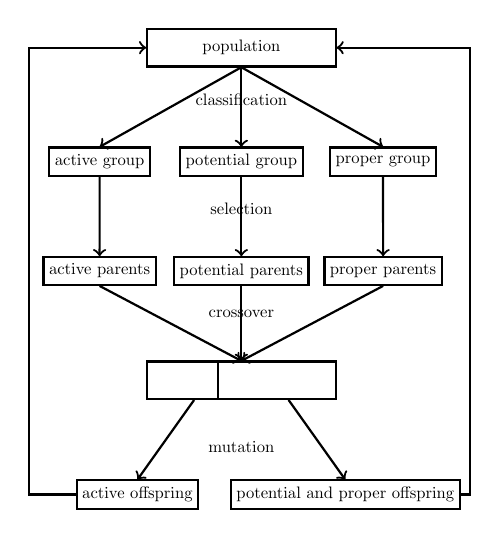
\begin{tikzpicture}[thick, scale=0.6, every node/.style={transform shape}]
	\tikzstyle{rec} = [rectangle, minimum width=4cm, minimum height=0.8cm,
	text centered, draw=black]
	\tikzstyle{subgroup} = [rectangle, minimum width=1.5cm, minimum height=0.6cm,
	text centered, draw=black]
	\tikzstyle{bigsubgroup} = [rectangle, minimum width=2.5cm, minimum height=0.6cm,
	text centered, draw=black]
	% population
	\node (population) [rec] {population};
	% active group
	\node (active_group_1) at ($(population.south)+(-3cm, -2.0cm)$) [subgroup]
		{active group};
	\node (active_group_2) at ($(active_group_1.south)+(0cm, -2.0cm)$)
		[subgroup] {active parents};
	\draw[->] (population.south) -- (active_group_1.north);
	\draw[->] (active_group_1.south) -- (active_group_2.north);
	% potential group
	\node (potential_group_1) at ($(population.south)+(0cm, -2.0cm)$) [subgroup]
		{potential group};
	\node (potential_group_2) at ($(potential_group_1.south)+(0cm, -2.0cm)$)
		[subgroup] {potential parents};
	\draw[->] (population.south) -- (potential_group_1.north);
	\draw[->] (potential_group_1.south) -- (potential_group_2.north);
	\node at ($(potential_group_1.north)+(0cm, 1.0cm)$) {classification };
	\node at ($(potential_group_2.north)+(0cm, 1.0cm)$) {selection};
    % proper group
	\node (proper_group_1) at ($(population.south)+(3cm, -2.0cm)$) [subgroup]
		{proper group};
	\node (proper_group_2) at ($(proper_group_1.south)+(0cm, -2.0cm)$)[subgroup]
		{proper parents};
	\draw[->] (population.south) -- (proper_group_1.north);
	\draw[->] (proper_group_1.south) -- (proper_group_2.north);
	% crossover
	\node (after_cross_over) at ($(potential_group_2.south)+(0cm, -2.0cm)$) [rec] {};
	\node  at ($(after_cross_over.north)+(0cm, 1.0cm)$)  {crossover};
	\draw[-] ($(after_cross_over.south)+(-0.5cm,0cm)$) --
		($(after_cross_over.north)+(-0.5cm,0cm)$);
	\draw[->] (active_group_2.south) -- (after_cross_over.north);
	\draw[->] (potential_group_2.south) -- (after_cross_over.north);
	\draw[->] (proper_group_2.south) -- (after_cross_over.north);
	% mutation
	\node (active_group_3) at ($(after_cross_over.south)+(-2.2cm, -2.0cm)$)
		[subgroup] {active offspring};
	\node at ($(after_cross_over.south)+(0cm, -1.0cm)$) {mutation};
	\draw[->] ($(after_cross_over.south)+(-1cm,0cm)$)--(active_group_3.north);
	\node (poteni_and_prop) at ($(after_cross_over.south)+(2.2cm, -2.0cm)$)
		[bigsubgroup] {potential and proper offspring};
	\draw[->] ($(after_cross_over.south)+(1cm,0cm)$)--(poteni_and_prop.north);

	% final draw
	\draw[->] (poteni_and_prop.east) --($(poteni_and_prop.east) + (0.2cm,0cm)$) |- (population.east);
	\draw[->] (active_group_3.west) -- ($(active_group_3.west) + (-1cm,0cm)$)
		|- (population.west);
\end{tikzpicture}
\end{center}
\caption{GA Model\label{GA:model}}
\end{figure}

\subsection{Genetic Algorithm}
The GA starts off with multiple individuals with limited chromosome lengths, in which maybe none of
these individuals fulfill the safety factor constraint. The GA is assumed to derive appropriate
offspring based on the initial population as the GA continues. The classic way to handle the constrained
search of the GA is either to introduce repair strategies or use a penalty function. Here, a new
approach is developed to address the constrained GA search problem by modifying the selection
strategy.

Because of the existence of constraints, the population can be sorted by the
fitness (which is obtained by the objective function) but can also be sorted by the constraint value
obtained by the constraint function (assuming a constraint function exists), so the parents of the next
generation can be chosen by the following two approaches. First, the population is sorted by the
absolute difference between the individual's constraint value and the threshold of the constraint in
ascending order, and individuals with smaller differences are more likely to be chosen. Individuals
obtained by this method are called potential individuals. Second, the population is sorted by fitness
from low to high after removing improper individuals, an individual is proper if it
fulfills the constraint, and individuals obtained in this way are called proper individuals. So the
final parents consists of two parts, potential individuals and proper individuals, and the number of
potential individuals and proper individuals are called, respectively, potential numbers and proper
number. For example, assuming the parent population is 20, 60 percent of are potential
individuals, and the rest are proper individuals. So the potential number is 12, and the proper
number is 8.

At the beginning of the GA, no individual in the population is appropriate, which means the number
of proper individuals is nearly zero. Therefore, the GA can be divided into two stages according to whether
proper individuals are generated during the search process. During the initial stages, the number of
potential individuals gradually decreases from the maximum (which is the parent population) to the potential
number, while the number of proper individuals increases from zero to the proper number as the GA
continues. After the initial stage, both groups converge to the
potential number and proper number. To differentiate the current selection methods from
the following, the current GA is called the basic GA. In the following experiment, 50 percent of the
parents are potential individuals, and 50 percent of the parents are proper individuals.

The problem with this basic GA is premature and has weak local search ability; therefore, basic GAs are more likely
to get stuck in a local optimum. Therefore, to prevent the GA from experiencing early convergence and to improve the
local search performance, a new selection method is proposed, which ignores whether the
individuals satisfy the constraint or not and ranks individuals by their fitness. Individuals
selected by this method are called active individuals because they are assumed to always be in the
population. GAs with these active individuals are called improved GAs. In the improved GA, the parents
consist of three parts: active individuals, potential individuals, and proper individuals. In the
following experiment, 20 percent of the parent population are active individuals, 30 percent of the
parents are potential individuals, and the rest are proper individuals.

In the present study, the relevant parameters of the GA are shown in Table \ref{tab:ga}. The design
variables are the materials, number of layers, and ply orientation restricted to a discrete set of
angles ($0,\pm 45 \text{ and } 90 \text{ degrees} $). The possible materials are graphite/epoxy,
carbon/epoxy, and glass/epoxy and are represented by codes 0, 1 and 2, respectively.


\begin{table}[!ht]
\centering
\caption{GA parameters}
\begin{adjustbox}{width=0.45\textwidth}
\label{tab:ga}
\begin{tabular}{cc}
\toprule
Parameter				&  Value  \\
\midrule
Seed					& 1       \\
Population size			& 20      \\
Initial length range	& [3-15]  \\
Encoding				& Integer  \\
Crossover strategy		& One-point \\
Mutation strategy		& Mass mutation \\
\bottomrule
\end{tabular}
\end{adjustbox}
\end{table}

%\begin{figure*}[!htb]
%  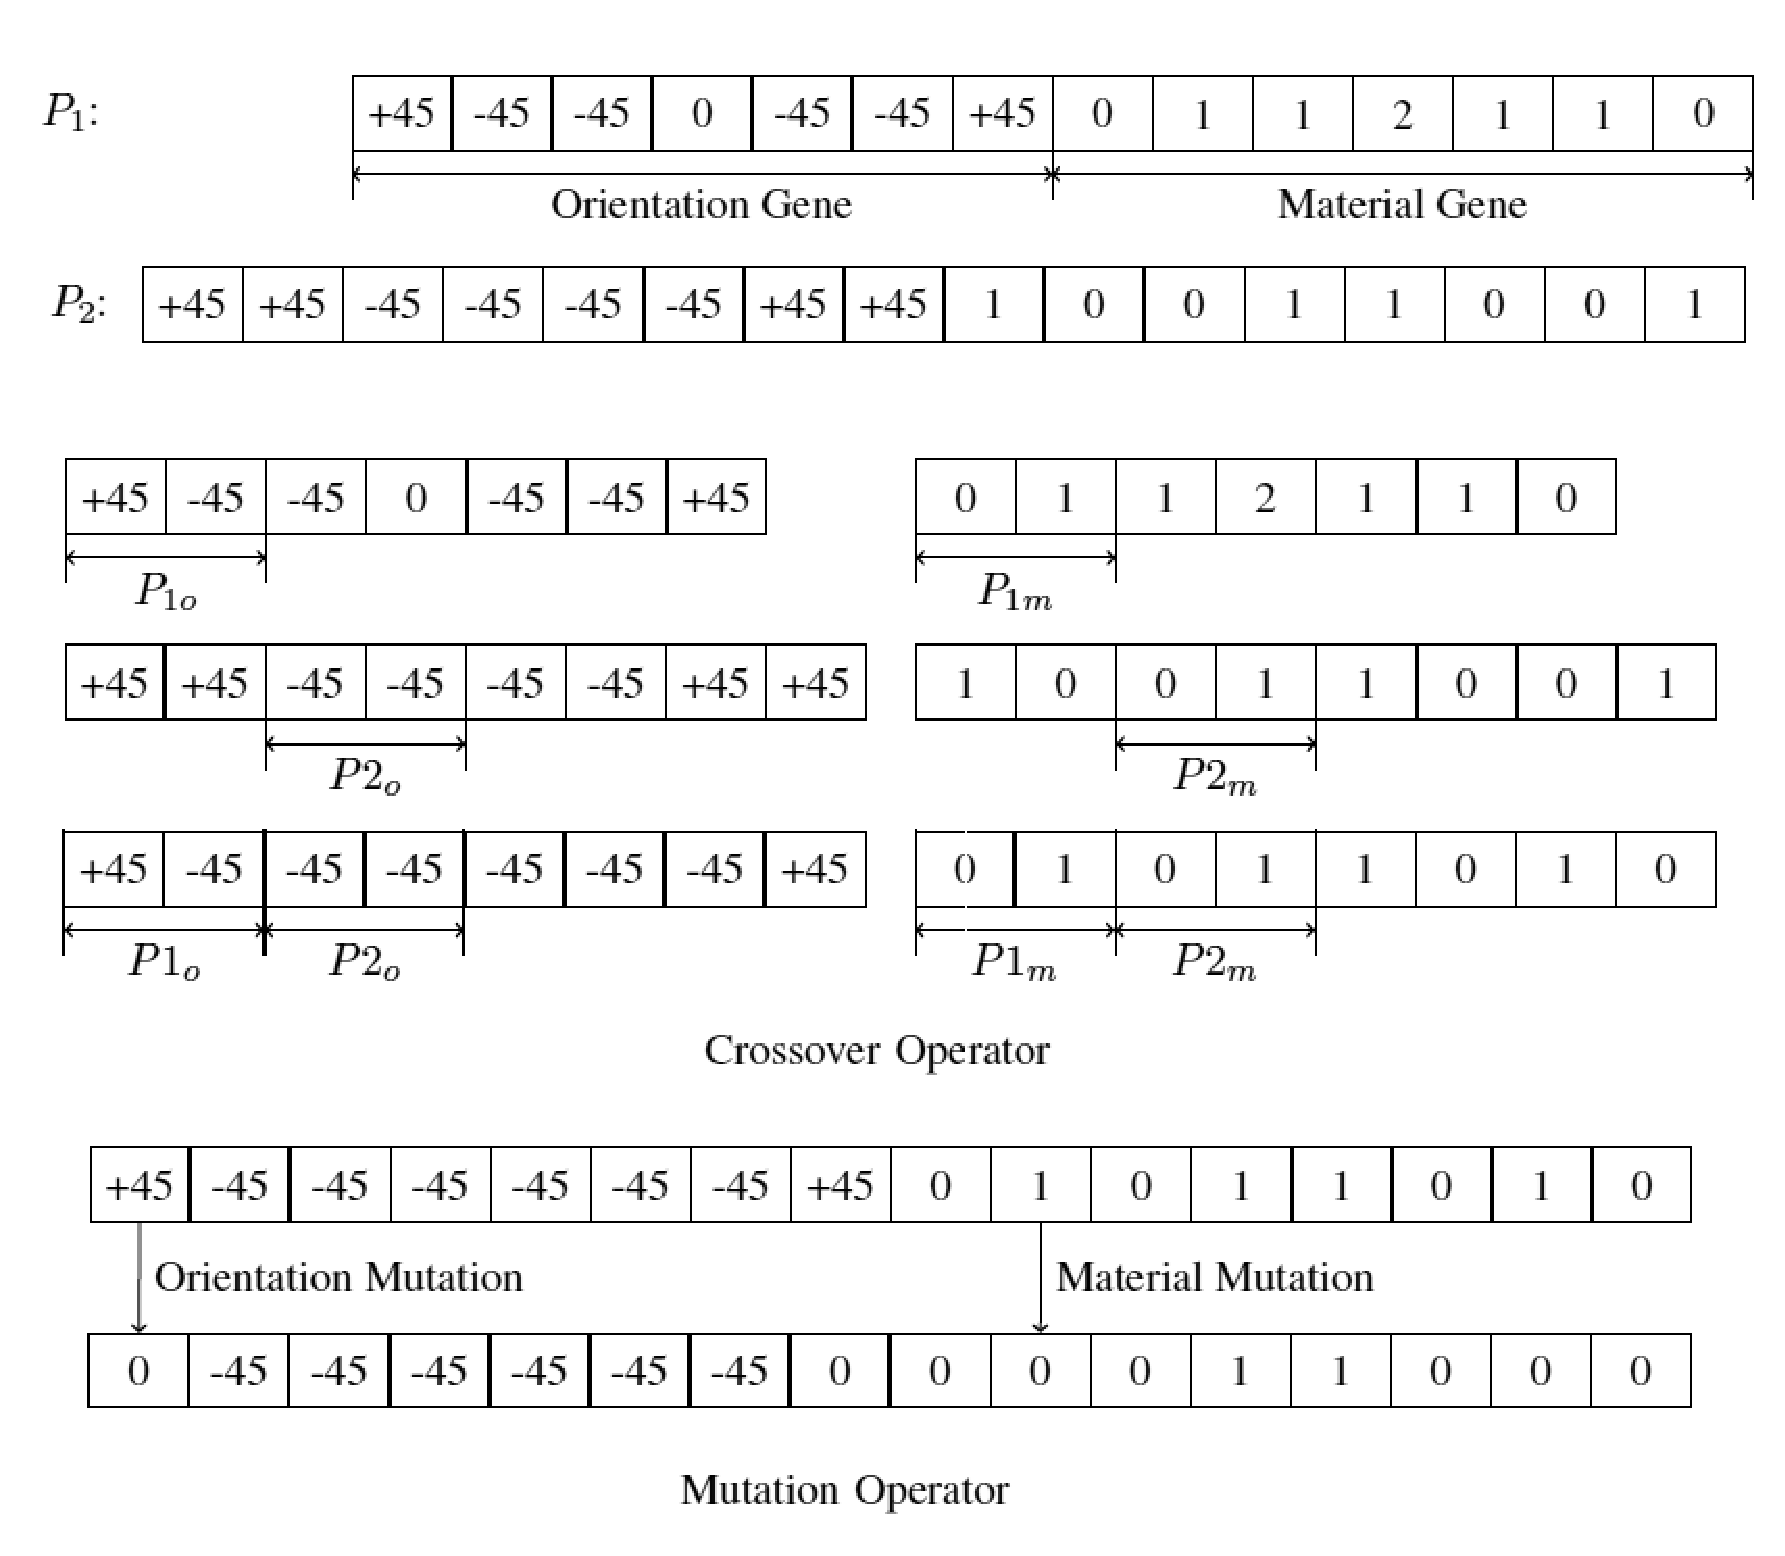
\includegraphics[width=\linewidth]{ga_operator}
%\caption{GA Operators\label{GA:operator}}
%\end{figure*}

The laminate chromosome is represented by a double-gene string that can be divided into two parts:
one part represents the angles, and the other part represents the materials (as shown in Figure
\ref{GA:operator}($P_1$)) . To maintain the diversity of the population, single-point crossover is
taken during the evolution process. The break points in the string are randomly chosen, and one of
the offspring of parent 1 (as shown in Figure \ref{GA:operator}($P_1$)) and parent 2 (as shown in
Figure \ref{GA:operator}($P_2$)) is obtained by combining the gene segments $P1_o$ and $P2_o$ and
$P1_m$ and $P2_m$, respectively. The gene code of the offspring laminate is
$[\text{+}45,\text{-}45,\text{-}45,\text{-}45,\text{-}45,\text{-}45,\text{-}45,0,1,0,1,1,0,1,0]$.


To prevent the search from becoming stuck in a local optimum, mutation is used to randomly change the
gene in the chromosome, and the offspring after the mutation operator is as shown in Figure
\ref{GA:operator}

The GA is a stochastic procedure that heavily depends on the generator of pseudorandom numbers. In
the present study, the standard Wichmann-Hill generator is used in the algorithm, which combines
three pure multiplicative congruent generators of moduli 30269, 30307 and 30323. The seed used
in this paper is 1.

\subsection{Design Problem I}

The aim is to minimize the mass of a laminate composite for a targeted strength
ratio based on the Tsai-wu failure theory. The design variable are the ply angles and the
number of layers.

Find: $\{\theta_k, n\}$ $\theta_k \in \{ 0,\text{+}45,\text{-}45,90\}$

Minimize: weight

Subject to: strength ratio and first ply failure constraint


\subsection{Design Problem II}
The aim is to minimize the weighted cost and weight of hybrid composite
laminates under various loading cases, so the design variable not only includes
the ply angles and number of layers but also the material of each lamina.


Find: $\{\theta_k,\text{mat}_k, n\}$ $\theta_k \in \{ 0,\text{+}45,\text{-}45,90\}$ $\text{mat}_k \in \{CA, GR, GL \}$

Minimize:
\begin{equation}
	F=\frac{\text { Cost }}{C_{\text {min }}}+\frac{\text { Weight }}{W_{\text {min }}}
\end{equation}

Subject to: strength ratio and first ply failure constraint


Here, CA, GF, and GL represent carbon/epoxy, graphite/epoxy, and glass/epoxy, and
$C_{\text{min}}$ and $W_{\text{min}}$ represent the cost and
weight corresponding to the laminates with a minimum cost and minimum weight
obtained from previous problem.

\section{Numerical Results and Discussion}
A laminate composite with dimensions $1000 \times 1000 \times 0.165 mm^3$ for
each lamina is under various loading cases, and each CA, GF, and GL layer is
assumed to cost 8, 2.5 and 1 monetary units, respectively. The other
material properties are shown in Table \ref{tab:mat}. A carbon/epoxy ply is represented by "cr", a
graphite/epoxy ply by "gl", and a glass/epoxy ply by "gl".  In the present
experiment, the optimal composite system, layup, thickness, and number of
layers for a targeted strength ratio (2 in this paper) under two different
in-plane loading conditions is investigated.

\begin{table*}[ht]
\caption{Comparison of the carbon/epoxy, graphite/epoxy, and glass/epoxy properties}
\centering
\begin{adjustbox}{width=1\textwidth}
\label{tab:mat}
\begin{tabular}{cccccc}
\toprule
Property								   & Symbol				  & Unit  &  Carbon/Epoxy&  Graphite/Epoxy  &  Glass/Epoxy   \\
\midrule
Longitudinal elastic modulus			   & $E_1$				  & GPa   &  116.6       &  181             &  38.6           \\
Traverse elastic modulus				   & $E_2$				  & GPa   &  7.67        &  10.3            &  8.27           \\
Major Poisson's ratio					   & $v_{12}$			  &       &  0.27        &  0.28            &  0.26           \\
Shear modulus							   & $G_{12}$			  & GPa   &  4.17        &  7.17            &  4.14           \\
Ultimate longitudinal tensile strength     & $(\sigma_1^T)_{ult}$ & MP    &  2062        &  1500            &  1062            \\
Ultimate longitudinal compressive strength & $(\sigma_1^C)_{ult}$ & MP    &  1701        &  1500            &  610             \\
Ultimate transverse tensile strength       & $(\sigma_2^T)_{ult}$ & MPa   &  70          &  40              &  31              \\
Ultimate transverse compressive strength   & $(\sigma_2^C)_{ult}$ & MPa   &  240         &  246             &  118              \\
Ultimate in-plane shear strength           & $(\tau_{12})_{ult}$  & MPa   &  105         &  68              &  72               \\
Density                                    & $\rho$               & $g/cm^3$ &  1.605    &  1.590           &  1.903               \\
Cost                                       &                      &       &  8           &  2.5             &  1               \\
\bottomrule
\end{tabular}
\end{adjustbox}
\end{table*}

%\begin{figure*}[!htb]
%	\centering
%	\includegraphics[width=\linewidth]{lamina_local_global_axes.eps}
%\caption{Lamina}
% 	\label{fig:lamina}
%\end{figure*}



\begin{table*}[!htb]
\caption{The optimum lay-ups for the loading $N_x=1e6$ N}
\centering
\begin{adjustbox}{width=1\textwidth}
\begin{tabular}{c|cc|cc}
	\toprule
	Cross Ply $[0_M/90_N]$         & \multicolumn{2}{c}{Previous Research} & \multicolumn{2}{c}{Current Research} \\
	\midrule																								  
	 Material       &  Glass-Epoxy & Graphite-Epoxy  & Glass-Epoxy & Graphite-Epoxy      \\ 
	      M         &  68          &    17           &  78		    &  18             \\
	      N         &  72          &    18           &  28		    &  8              \\
no. of lamina(n)    &  140         &    35           &  106	    &  26                     \\
         SR         &  2.01        &    2.10         &  2.03	    &  2.16            \\
     weight         &  9.10        &    1.84         &  6.89	    &  102.5           \\
	\bottomrule
\end{tabular}
\end{adjustbox}
\label{tab:comparsion}
\end{table*}



The GA process can be divided into two phases by whether there are individuals that are appropriate
or not. During the initial phase, no individual's strength ratio is over the specified threshold, so
individuals with larger fitness are more likely to be chosen as parents, which is why the strength
ratio curves go all the way up to the specified threshold during the first stage. After the initial
phase, the GA produces many appropriate individuals, and then the target function is utilized, and
as shown in Fig. \ref{fig:NxNy}, the fitness curves tend to decrease, but the
strength ratio curves remain greater than the specified threshold.

\begin{table*}[!htb]
\caption{The optimum lay-ups for the loading $N_x=N_y=1e6$ N}
\centering
\begin{adjustbox}{width=1\textwidth}
\begin{tabular}{cccccc}
	\toprule
	 Problem  &    Stacking sequence                                    & Strength ratio  & Mass  &  Cost   & Layer    \\ 
	\midrule																								  
	      I   &  $[\text{-}45_{6}^{cr}/\text{+}45_{6}^{cr}]_s$                        & 2.026           & 1.271 &  192.0  & 24  \\
	      I   &  $[\text{+}45_{10}^{gr}/\text{-}45_{10}^{gr}/\bar{\text{-}45}^{gr}]_s$    & 2.024           & 2.151 &  102.5  & 41  \\
	      I   &  $[\text{-}45_{35}^{gl}/\text{+}45_{36}^{gl}/\bar{\text{+}45}^{gl}]_s$    & 2.001           & 8.980 &  143.0  & 143  \\
	      II  & $[\text{-}45_{9}^{gr}/\text{+}45_{9}^{gr}/\text{-}45_{2}^{cr}/\text{+}45_{2}^{cr}]_s$         & 2.054
										  & 2.313 & 154& 44  \\
	\bottomrule
\end{tabular}
\end{adjustbox}
\label{tab:NxNy}
\end{table*}


In the first experiment, the applied stress is $N_x=N_y=1e6$ N. As shown in
Figure \ref{fig:NxNy}, Figures \ref{fig:NxNy}(a), (b), and (c) show the experimental results for a single material,
Figure \ref{fig:NxNy}(d) shows the results for the hybrid composite material.
 For the single materials, both the basic GA and improved
GA method obtained the optimal value, but the improved GA converged more slowly than the basic GA.
As seen from Table \ref{tab:NxNy}, a $[\text{-}45_{6}/\text{+}45_{6}]_s$ carbon/epoxy
laminate has the least weight, denoted by $W_{min}$, and a
$[\text{-}45_{35}/\text{+}45_{73}/\text{+}45_{35}]$ graphite/epoxy laminate has the lowest cost,
denoted by $C_{min}$. $W_{min}$ and $C_{min}$ were used to evaluate the fitness of the second
problem, which is the layup design of the hybrid composite material. As shown in subfigure d, the
improved GA obtained a more appropriate system layup, whose strength ratio was greater than the
specified safety factor, and the weight and cost are less than the result obtained by the basic GA method, as
shown in Table \ref{tab:NxNy}.
 Compared with the basic GA, the improved GA method showed more powerful
global search ability in the initial phase.

\begin{table*}[!htb]
\caption{The optimum lay-ups for the loading $N_x=N_y=1e6$ N}
\centering
\begin{adjustbox}{width=1\textwidth}
\begin{tabular}{cccccc}
	\toprule
	 Problem  &    Stacking sequence                                    & Strength ratio  & Mass  &  Cost   & Layer    \\ 
	\midrule																								  
	      I   &  $[\text{-}45_{6}^{cr}/\text{+}45_{6}^{cr}]_s$                        & 2.026           & 1.271 &  192.0  & 24  \\
	      I   &  $[\text{+}45_{10}^{gr}/\text{-}45_{10}^{gr}/\bar{\text{-}45}^{gr}]_s$    & 2.024           & 2.151 &  102.5  & 41  \\
	      I   &  $[\text{-}45_{35}^{gl}/\text{+}45_{36}^{gl}/\bar{\text{+}45}^{gl}]_s$    & 2.001           & 8.980 &  143.0  & 143  \\
	      II  & $[\text{-}45_{9}^{gr}/\text{+}45_{9}^{gr}/\text{-}45_{2}^{cr}/\text{+}45_{2}^{cr}]_s$         & 2.054
										  & 2.313 & 154& 44  \\
	\bottomrule
\end{tabular}
\end{adjustbox}
\label{tab:NxNy}
\end{table*}


In the second case, the applied stress was $N_x=N_y=N_z=1e6$ N, and the experimental results were as
shown in the Figure \ref{fig:NxNyNz}. In the first experiment, as seen from Figure \ref{fig:NxNyNz}(a), the improved GA obtained a
better system layup than the result obtained by the basic GA. In the second experiment, as shown in Figure \ref{fig:NxNyNz}(b), during
the initial phase, the fitness curves of the basic GA and improved GA went all the way up to the
previous specified threshold; however, the improved GA converged more slowly than the basic GA, which
means that the search cost of the improved GA was greater than that of the basic GA. After the initial phase, the fitness
curve of the basic GA did not change anymore, it got trapped in the local domain.
 However, the fitness curve of the
improved GA gradually decreased; at the same time, the strength ratio curve of the improved GA
was maintained to be greater than the threshold. This means the improved GA was able to get out of the optimum
and obtain a much better system layup. The improved GA offered more powerful local search
ability. In the third experiment, as shown in Figure \ref{fig:NxNyNz}, both the basic GA and improved
GA obtained the same result, but the improved GA converged more slowly than the basic GA. From these
three experiments for a single material, we know that a $[\text{+}45_{6}^{cr}]_s$ carbon/epoxy laminate has
the least mass, and a $[\text{+}45_{11}^{gl}/\bar{\text{+}45}^{gl}]_s$ glass laminate has the least
cost. In the last experiment, the improved GA obtained a slightly better result than the basic GA,
as shown in Table \ref{tab:NxNyNz}. Compared with the $[\text{+}45_{12}^{cr}]$ laminate, the
weight of a $[\text{+}45_8^{gr}/\bar{\text{+}45}^{gl}]_s$ laminate increased $41.8\%$, however, the
cost decreased $56\%$.


\section{Conclusions}
In this paper, a combination of CLT and a variant of the GA are employed to minimize the weight and cost
of a single-material and hybrid composite laminate, respectively, under various in-plane loading
cases. The results are presented in two sections: stacking sequence optimization for a single material
laminate, and weighted mass and cost optimization of a carbon/epoxy, graphite/epoxy, and
glass/epoxy hybrid laminates. Furthermore, the performance of the basic GA is improved by changing the
selection strategy.

This variant of the GA provides a new approach to address the search constraint in laminate composite
optimization, and this method is very easy to extend for solving the multiple constraint search problem in other
domain. The problem with the current method involves adjusting the parameters in the GA to obtain the best
performance.

\begin{acks}
Huiyao Zhang is grateful for the financial support from the China Scholarship Council(201806630112)
\end{acks}

\bibliographystyle{SageV}
\bibliography{reference}

\end{document}
